%% LyX 2.0.2 created this file.  For more info, see http://www.lyx.org/.
%% Do not edit unless you really know what you are doing.
\documentclass[10pt,english]{beamer}
\usepackage{mathptmx}
\usepackage[T1]{fontenc}
\usepackage[latin9]{inputenc}
\usepackage{color}
\usepackage{babel}
\usepackage{array}
\usepackage{amsmath}
\usepackage{amssymb}
\usepackage{graphicx}
\ifx\hypersetup\undefined
  \AtBeginDocument{%
    \hypersetup{unicode=true,
 bookmarks=true,bookmarksnumbered=false,bookmarksopen=false,
 breaklinks=true,pdfborder={0 0 1},backref=false,colorlinks=true,pdftitle={TopSVDFunctions - Reference},
 pdfauthor={David J. Fischer},
 hyphens}
  }
\else
  \hypersetup{unicode=true,
 bookmarks=true,bookmarksnumbered=false,bookmarksopen=false,
 breaklinks=true,pdfborder={0 0 1},backref=false,colorlinks=true,pdftitle={TopSVDFunctions - Reference},
 pdfauthor={David J. Fischer},
 hyphens}
\fi

\makeatletter

%%%%%%%%%%%%%%%%%%%%%%%%%%%%%% LyX specific LaTeX commands.
%% Because html converters don't know tabularnewline
\providecommand{\tabularnewline}{\\}

%%%%%%%%%%%%%%%%%%%%%%%%%%%%%% Textclass specific LaTeX commands.
 % this default might be overridden by plain title style
 \newcommand\makebeamertitle{\frame{\maketitle}}%
 \AtBeginDocument{
   \let\origtableofcontents=\tableofcontents
   \def\tableofcontents{\@ifnextchar[{\origtableofcontents}{\gobbletableofcontents}}
   \def\gobbletableofcontents#1{\origtableofcontents}
 }
 \long\def\lyxframe#1{\@lyxframe#1\@lyxframestop}%
 \def\@lyxframe{\@ifnextchar<{\@@lyxframe}{\@@lyxframe<*>}}%
 \def\@@lyxframe<#1>{\@ifnextchar[{\@@@lyxframe<#1>}{\@@@lyxframe<#1>[]}}
 \def\@@@lyxframe<#1>[{\@ifnextchar<{\@@@@@lyxframe<#1>[}{\@@@@lyxframe<#1>[<*>][}}
 \def\@@@@@lyxframe<#1>[#2]{\@ifnextchar[{\@@@@lyxframe<#1>[#2]}{\@@@@lyxframe<#1>[#2][]}}
 \long\def\@@@@lyxframe<#1>[#2][#3]#4\@lyxframestop#5\lyxframeend{%
   \frame<#1>[#2][#3]{\frametitle{#4}#5}}
 \def\lyxframeend{} % In case there is a superfluous frame end

%%%%%%%%%%%%%%%%%%%%%%%%%%%%%% User specified LaTeX commands.
\usepackage{multicol}
\usetheme{Madrid} 
\usecolortheme{orchid} 
\setbeamercovered{transparent} 
\setbeamertemplate{navigation symbols}{} 
% DEFINE YOUR LOGO
\newcommand{\mylogo}{
 
\includegraphics[width=1cm,height=1cm,keepaspectratio]{./Desylogo.pdf}~%
 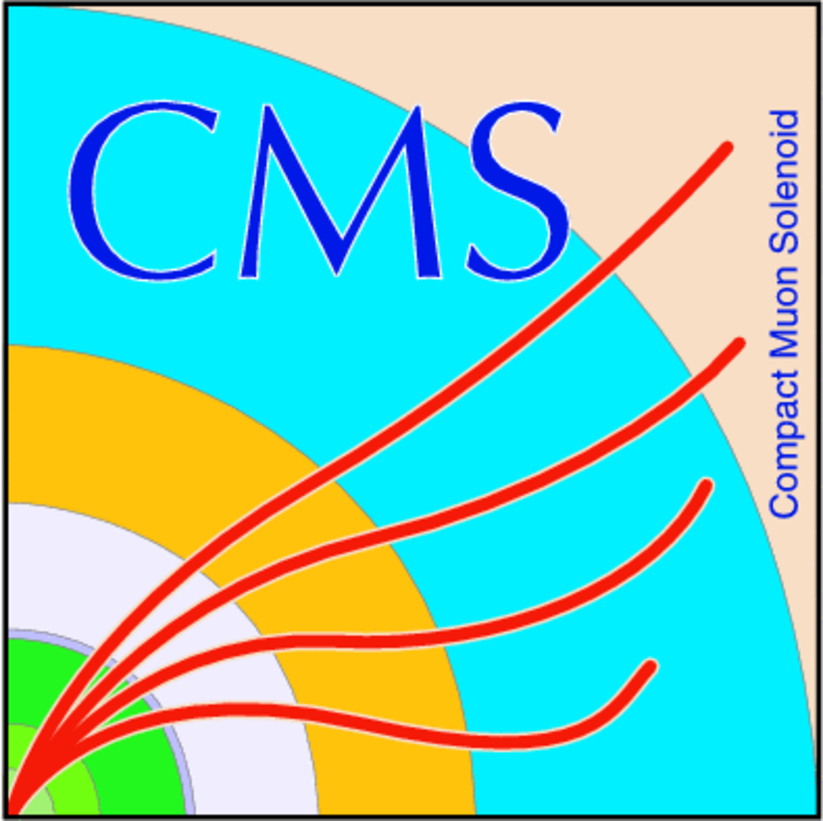
\includegraphics[width=1cm,height=1cm,keepaspectratio]{./CMSlogo.pdf}%
}

\usepackage{url}
 

% OVERWRITE FRAME DEFINITION
\let\oldlyxframe\lyxframe 
\renewcommand{\lyxframe}[1]{\oldlyxframe{\mylogo\hspace{3mm} #1}}


\setbeamersize{text margin left=1cm,text margin right=1cm} 

\makeatother

\begin{document}

\title{TopSVDFunctions}


\subtitle{Reference Guide}


\author{D.~J.~Fischer\inst{1}}


\institute{\inst{1}DESY Hamburg}


\date[9/17/2012]{September 17, 2012}

\makebeamertitle

\lyxframeend{}\lyxframe{What is TopSVDFunctions?}
\begin{itemize}
\item TopSVDFunctions is a C++ class, providing unfolding functionality.
\item It is designed with two specific CMS analyses in mind, which are

\begin{itemize}
\item the DESY top quark pair production cross section measurement in the
dilepton channel and
\item the Uni-HH top quark pair production cross section measurement in
the semileptonic channel. 
\end{itemize}
\item \textbf{The whole design is optimized to fulfill the specific needs
of those two analyses!}
\end{itemize}

\lyxframeend{}


\lyxframeend{}\lyxframe{Key Features}
\begin{itemize}
\item \textbf{SVD unfolding}\textbf{\emph{ }}based on $\texttt{ROOT-}$class
$\texttt{TSVDUnfold}$ by Kerstin Tackmann.
\item \textbf{Adjustment of regularization }based on the global correlation
method ($\tau$-parameter scan).
\item An \textbf{easy to use interface}. The user has to get acquainted
with just one function call!
\item A lot of unfolding related \textbf{control plots}.
\item Error propagation of\textbf{ statistical and systematic uncertainties}.
\end{itemize}

\lyxframeend{}


\lyxframeend{}\lyxframe{Supplemental Features}
\begin{itemize}
\item \textbf{Background removal}\textbf{\emph{ }}based on a combination
of a simple \emph{subtraction method} and the \emph{signal fraction
method}. (Explained later in this reference guide.)
\item \textbf{Rebinning} of input histograms.
\item \textbf{Iterative unfolding}: Reweight your MC to the unfolded data
and unfold again.
\item Simple \textbf{closure test}\textbf{\emph{: }}Test the method by unfolding
your MC distribution. 
\end{itemize}

\lyxframeend{}


\lyxframeend{}\lyxframe{Notes on SVD Unfolding}
\begin{itemize}
\item TopSVDFunctions uses the ROOT class TSVDUnfold to do the actual unfolding.

\begin{itemize}
\item For documentation, see ROOT class reference.
\end{itemize}
\item The method is described in the paper by Andreas Hoecker and Vakhtang
Kartvelishvili: \url{http://arxiv.org/abs/hep-ph/9509307}
\item An introduction into the mathematical aspects of the method was given
March 20, 2012: \url{https://indico.desy.de/getFile.py/access?contribId=1&resId=0&materialId=slides&confId=5440}
\end{itemize}

\lyxframeend{}\lyxframe{Where is the code?}
\begin{itemize}
\item CVS directory: \url{http://cmssw.cvs.cern.ch/cgi-bin/cmssw.cgi/UserCode/Bromo/TopAnalysis/Configuration/analysis/unfolding/}
\item Note: This is a common CVS directory of DESY and Uni-HH! 
\end{itemize}

\lyxframeend{}


\lyxframeend{}\lyxframe{What files are involved?}

\begin{center}
\begin{tabular}{|>{\centering}p{4cm}|>{\centering}p{6cm}|}
\hline 
Files & Function\tabularnewline
\hline 
\hline 
TopSVDFunctions.h/C & Main class of this package.\tabularnewline
\hline 
BaseSVDUnfold.h/C & Contains ROOT-class TSVDUnfold by Kerstin Tackmann, renamed to BaseSVDUnfold.\tabularnewline
\hline 
TopSVDUnfold.h/C & Derives from BaseSVDUnfold, adding functionality needed by TopSVDFunctions. \tabularnewline
\hline 
CP\_booklet & Folder with shell scripts to create \LaTeX{} booklets with control
plots.\tabularnewline
\hline 
Documentation & Folder with documentation.\tabularnewline
\hline 
\end{tabular}
\par\end{center}


\lyxframeend{}


\lyxframeend{}\lyxframe{Dependencies}
\begin{itemize}
\item C/C++ standard library and STL 
\item ROOT

\begin{itemize}
\item Version used for developement and testing: ROOT 5.27
\item No reference to TSVDUnfold! We use a direct copy of TSVDUnfold renamed
to BaseSVDUnfold.
\end{itemize}
\item UniHH functions

\begin{itemize}
\item CVS directory: \url{http://cmssw.cvs.cern.ch/cgi-bin/cmssw.cgi/UserCode/Bromo/TopAnalysis/Configuration/analysis/semiLeptonic/diffXSection}
\end{itemize}
\item Code \textbf{does not}\textbf{\emph{ }}\textbf{depend on CMSSW} in
any way!
\end{itemize}

\lyxframeend{}


\lyxframeend{}\lyxframe{Installation}
\begin{itemize}
\item Make sure that ROOT, C/C++ standard lib and STL is available.
\item Download unfolding code from CVS
\item Download UniHH functions from CVS 
\item If you are running a ROOT macro, use 
\[
\texttt{\#include TopSVDFunctions.C}
\]
at the top of your source file. Or, if you are using executable files,
use
\[
\texttt{\#includeTopSVDFunctions.h}
\]
and adapt your Makefile accordingly.
\item You are ready to call the function 
\[
\texttt{TopSVDFunctions::SVD\_Unfold(...)}
\]
 from your code.
\end{itemize}

\lyxframeend{}


\lyxframeend{}\lyxframe{The Interface - Overview}
\begin{itemize}
\item Everything goes through \textbf{one static function}\emph{:}
\[
\texttt{TopSVDFunctions::SVD\_Unfold(...)}
\]
 
\item That means: Exactly one place of interaction with the code! 

\begin{itemize}
\item No setting of environment variables needed.
\item No setting of data members needed. (In fact, there are none.)
\end{itemize}
\end{itemize}

\lyxframeend{}


\lyxframeend{}\lyxframe{The Interface - Overview}

\texttt{\footnotesize static double SVD\_Unfold(}{\footnotesize \par}

\texttt{\footnotesize TH1D{*} dataInputHist, TH1D{*} bgrInputHist,
TH1D{*} ttbgrInputHist, TH1D{*} genInputHist, TH1D{*} recInputHist,
TH2D{*} respInputHist, TH1D{*}\& unfolded, TH1D{*}\& unfoldedNorm,
double{*} totalDataEvents, double{*} totalBgrEvents, double{*} totalTtBgrEvents,
double{*} totalRecEvents, double{*} totalGenEvents, const double thebins{[}{]},
const int numbins, double regPar, TString steering = \textquotedbl{}\textquotedbl{},
const int numSys = 0, TString channel = \textquotedbl{}\textquotedbl{},
TString particle = \textquotedbl{}\textquotedbl{}, TString quantity
= \textquotedbl{}\textquotedbl{}, TString special = \textquotedbl{}\textquotedbl{},
TString systname = \textquotedbl{}\textquotedbl{}, TString channelTex
= \textquotedbl{}\textquotedbl{}, TString particleTex = \textquotedbl{}\textquotedbl{},
TString quantityTex = \textquotedbl{}\textquotedbl{}, TString specialTex
= \textquotedbl{}\textquotedbl{}, TString systnameTex = \textquotedbl{}\textquotedbl{},
TString rootFile = \textquotedbl{}\textquotedbl{}, TString psFile
= \textquotedbl{}\textquotedbl{}, TString epsFile = \textquotedbl{}\textquotedbl{},
TString txtFile = \textquotedbl{}\textquotedbl{}, TString regParFile
= \textquotedbl{}\textquotedbl{} ); }{\footnotesize \par}


\lyxframeend{}


\lyxframeend{}\lyxframe{The Interface - Data Input }
\begin{itemize}
\item \textbf{TH1D{*} dataInputHist}

\begin{itemize}
\item Raw data distribution \emph{before} background removal. 
\item Expected to be a single histogram (array of length 1).
\end{itemize}
\item \textbf{double{*} totalDataEvents}

\begin{itemize}
\item Total event count \emph{before} background removal. 
\item Expected to be a single double (array of length 1). If a NULL pointer
is given, the value is assumed to be the integral of dataInputHist.
\end{itemize}
\end{itemize}

\lyxframeend{}


\lyxframeend{}\lyxframe{The Interface - Signal Input}
\begin{itemize}
\item \textbf{TH1D{*} genInputHist}

\begin{itemize}
\item The generator level signal MC distribution.
\item The distribution must have all generator level weights applied, in
particular the luminosity weight.
\item Expected to be an array of length numSys+1. 
\item Tip: If you want, you can impose cuts on this distribution, such as
phase space cuts, which will be propagated to the unfolding result.
\end{itemize}
\item \textbf{double{*} totalGenEvents} 

\begin{itemize}
\item Total event count of generator level signal MC events.
\item The value must have all generator level weights applied, in particular
the luminosity weight.
\item Expected to be an array of length numSys+1. If a NULL pointer is given,
the value is assumed to be the integral of genInputHist. 
\end{itemize}
\end{itemize}

\lyxframeend{}


\lyxframeend{}\lyxframe{The Interface - Signal Input}
\begin{itemize}
\item \textbf{TH1D{*} recInputHist}

\begin{itemize}
\item The reconstruction level signal MC distribution. 
\item The distribution must have all generator level and reconstruction
level weights applied, in particular the luminosity weight.
\item Expected to be an array of length numSys+1.
\end{itemize}
\item \textbf{double{*} totalRecEvents }

\begin{itemize}
\item Total event count of reconstruction level signal MC events. 
\item The value must have all generator level and reconstruction level weights
applied, in particular the luminosity weight.
\item Expected to be an array of length numSys+1. If a NULL pointer is given,
the value is assumed to be the integral of recInputHist. 
\end{itemize}
\end{itemize}

\lyxframeend{}


\lyxframeend{}\lyxframe{The Interface - Signal Input}
\begin{itemize}
\item \textbf{TH1D{*} respInputHist}

\begin{itemize}
\item Response matrix. Entries are expected to be event counts from signal
MC (\emph{Event Matrix}). 
\item The distribution must have all generator level and reconstruction
level weights applied, in particular the luminosity weight.
\item Expected to be an array of length numSys+1.
\item Orientation:

\begin{itemize}
\item Reconstruction level quantities are expected on the x-Axis and generator
level quantities on the y-Axis.
\item If a different orientation is given, you can transpose the matrix
with the steering option number 12, see below. 
\end{itemize}
\end{itemize}
\end{itemize}

\lyxframeend{}


\lyxframeend{}\lyxframe{The Interface - Background Input}
\begin{itemize}
\item \textbf{TH1D{*} bgrInputHist: }

\begin{itemize}
\item Distribution of the complete simulated background (reconstruction
level) to be removed from the data. 
\item The distribution must have all generator level and reconstruction
level weights applied, in particular the luminosity weight.
\item If a NULL pointer is given, no background will be removed. 
\end{itemize}
\item \textbf{double{*} totalBgrEvents}

\begin{itemize}
\item Total event count of simulated background (reconstruction level) to
be removed from the data. 
\item The value must have all generator level and reconstruction level weights
applied, in particular the luminosity weight.
\item If a NULL pointer is given, the value is assumed to be the integral
of bgrInputHist. If bgrInputHist is a NULL pointer, the value is assumed
to be 0.
\end{itemize}
\end{itemize}

\lyxframeend{}


\lyxframeend{}\lyxframe{The Interface - Background Input}
\begin{itemize}
\item \textbf{TH1D{*} ttbgrInputHist}

\begin{itemize}
\item Fraction of the simulated background (reconstruction level) which
will be removed by the \emph{Signal Fraction Method}.
\item The distribution must have all generator level and reconstruction
level weights applied, in particular the luminosity weight.
\item If a NULL pointer is given, the Signal Fraction Method will not be
used. 
\end{itemize}
\item \textbf{double{*} totalTtBgrEvents}

\begin{itemize}
\item Total event count of simulated background (reconstruction level) which
will be removed by the \emph{Signal Fraction Method}.
\item The value must have all generator level and reconstruction level weights
applied, in particular the luminosity weight.
\item If a NULL pointer is given, the value is assumed to be the integral
of ttbgrInputHist. If ttBgrInputHist is a NULL pointer, the Signal
Fraction Method will not be used. 
\end{itemize}
\end{itemize}

\lyxframeend{}


\lyxframeend{}\lyxframe{The Interface - Binning }
\begin{itemize}
\item \textbf{const int numbins}

\begin{itemize}
\item Number of bins used in the unfolding procedure (\emph{target} \emph{binning}).
\end{itemize}
\item \textbf{const double thebins{[}{]}}

\begin{itemize}
\item Bin boundaries of the binning used in the unfolding procedure (\emph{target
binning}). Expected to be an array of doubles with numbins+1 entries.
\end{itemize}
\end{itemize}

\lyxframeend{}


\lyxframeend{}\lyxframe{The Interface - Output }
\begin{itemize}
\item \textbf{TH1D{*}\& unfolded}

\begin{itemize}
\item Output histogram with unfolded data distribution. 
\item The \emph{output binning }will be used (see below). This means, the
first and last bin of the histogram are overflow bins. In particular,
while drawn with finite width, these bins may correspond to an infinite
range!
\end{itemize}
\item \textbf{TH1D{*}\& unfoldedNorm}

\begin{itemize}
\item Output histogram with normalized unfolded data distribution.
\item The \emph{output binning }will be used (see below). This means, the
first and last bin of the histogram are overflow bins. In particular,
while drawn with finite width, these bins may correspond to an infinite
range!
\end{itemize}
\end{itemize}

\lyxframeend{}


\lyxframeend{}\lyxframe{The Interface - Regularization }
\begin{itemize}
\item \textbf{double regPar}

\begin{itemize}
\item Regularization parameter. Can be given in two formats:

\begin{itemize}
\item \emph{k-Parameter}: regPar must take on an integer value between 1
and numBins (number of bins in the target binning). Set the second
steering option to 1. Examples:
\[
\texttt{double regPar = 2.0, double regPar = 8.0}
\]

\item $\tau$-\emph{Parameter:} regPar must take on a real value greater
than zero. Set the second steering option to 2.Examples:
\[
\texttt{double regPar = 1.630E-5, double regPar = 1.30E-2 }
\]

\end{itemize}
\item Will only be used, if the first steering option is set to 3, accordingly. 
\end{itemize}
\end{itemize}

\lyxframeend{}


\lyxframeend{}\lyxframe{The Interface - Systematics}
\begin{itemize}
\item \textbf{const int numSys = 0}

\begin{itemize}
\item All pointer type parameters are interpreted as \emph{arrays!}

\begin{itemize}
\item Idea: Process multiple samples with different systematic shifts at
the same time.
\end{itemize}
\item numSys steers the array length of all pointer type parameters.
\item All pointer type parameters will be expected to have length numSys+1.

\begin{itemize}
\item \emph{Exception}: TH1D{*} dataInputHist and double totalDateEvents
will always be interpreted as anarray of length $\texttt{1}$, as
there should be no systematic shifts on the raw data! 
\end{itemize}
\end{itemize}
\end{itemize}

\lyxframeend{}


\lyxframeend{}\lyxframe{The Interface - Naming of Distributions}
\begin{itemize}
\item \textbf{TString channel = \textquotedbl{}\textquotedbl{}}

\begin{itemize}
\item Name of the channel under investigation. Will be used in naming of
histograms and output files.
\end{itemize}
\item \textbf{TString particle = \textquotedbl{}\textquotedbl{}}

\begin{itemize}
\item Name of the physics object under investigation. Will be used in naming
of histograms and output files.
\end{itemize}
\item \textbf{TString quantity = \textquotedbl{}\textquotedbl{}}

\begin{itemize}
\item Name of the variable under investigation. Will be used in naming of
histograms and output files.
\end{itemize}
\item \textbf{TString special = \textquotedbl{}\textquotedbl{}}

\begin{itemize}
\item String to specify a special condition during this unfolding process.
Will be used in naming of histograms and output files.
\end{itemize}
\item \textbf{TString systname = \textquotedbl{}\textquotedbl{}}

\begin{itemize}
\item Name of the systematic shift under investigation. Will be used in
naming of histograms and output files.
\end{itemize}
\end{itemize}

\lyxframeend{}


\lyxframeend{}\lyxframe{The Interface - Legends and Axis Titles}
\begin{itemize}
\item \textbf{TString channelTex = \textquotedbl{}\textquotedbl{}}

\begin{itemize}
\item Tex string for the channel under investigation. Uses ROOT/\TeX{}-Syntax.
Will be used in legends and axis titles.
\end{itemize}
\item \textbf{TString particleTex = \textquotedbl{}\textquotedbl{}}

\begin{itemize}
\item Tex string for the physics object under investigation. Uses ROOT/\TeX{}-Syntax.
Will be used in legends and axis titles.
\end{itemize}
\item \textbf{TString quantityTex = \textquotedbl{}\textquotedbl{}}

\begin{itemize}
\item Tex string for the variable under investigation. Uses ROOT/\TeX{}-Syntax.
Will be used in legends and axis titles.
\end{itemize}
\item \textbf{TString specialTex = \textquotedbl{}\textquotedbl{}}

\begin{itemize}
\item Tex string to describe any special condition of this unfolding process.
Uses ROOT/\TeX{}-Syntax. Will be used in legends and axis titles.
\end{itemize}
\item \textbf{TString systnameTex = \textquotedbl{}\textquotedbl{}}

\begin{itemize}
\item Tex string for the systematic shift under investigation. Uses ROOT/\TeX{}-Syntax.
Will be used in legends and axis titles.
\end{itemize}
\end{itemize}

\lyxframeend{}


\lyxframeend{}\lyxframe{The Interface - Output Files}
\begin{itemize}
\item \textbf{TString rootFile = \textquotedbl{}\textquotedbl{}}

\begin{itemize}
\item Name of the ROOT file (including ending '.root') to contain all control
plots.
\item Will only be created, if steering option 5 is set to 2. 
\item Will only be breated, if rootFile is a valid file name.
\end{itemize}
\item \textbf{TString psFile = \textquotedbl{}\textquotedbl{}}

\begin{itemize}
\item Name of the PS File (including ending '.ps') to contain all control
plots.
\item Will only be created, if steering option 4 is set to 2, 3 or 4. 
\item Will only be created, if psFile is a valid file name. 
\end{itemize}
\end{itemize}

\lyxframeend{}


\lyxframeend{}\lyxframe{The Interface - Output Files}
\begin{itemize}
\item \textbf{TString epsFile = \textquotedbl{}\textquotedbl{}}

\begin{itemize}
\item String steering the names of the EPS files to contain all control
plots. 
\item The name will be extended by a descriptive suffix indicating the plot
content, thereby following the following pattern:

\begin{itemize}
\item If epsFile is set to '<myName>.eps', the actual file names will be
'<myName>\_<description>.eps'.
\item Example: If epsFile is set to 'Output.eps', one file will be named
'Output\_ResultUnfBbb.eps'.
\end{itemize}
\item Will only be created, if steering option 4 is set to 2, 3 or 4. 
\item Will only be created, if epsFile is a valid file name. 
\end{itemize}
\end{itemize}

\lyxframeend{}


\lyxframeend{}\lyxframe{The Interface - Regularization Parameter Files}
\begin{itemize}
\item \textbf{TString txtFile = \textquotedbl{}\textquotedbl{}}

\begin{itemize}
\item Output text file (including ending '.txt') containing the results
of a regularization parameter scan. 
\item Will only be created, if txtFile is a valid file name.
\end{itemize}
\item \textbf{TString regParFile = ``''}

\begin{itemize}
\item Input text file (including ending '.txt') with the input regularization
parameters.
\item Will only be used, if the first steering option is set to 3, accordingly. 
\end{itemize}
\end{itemize}

\lyxframeend{}


\lyxframeend{}\lyxframe{The Interface - Steering Options}
\begin{itemize}
\item \textbf{TString steering}

\begin{itemize}
\item This TString type parameter takes integer digits, steering the behaviour
of the unfolding process.
\item Each digit represents one \textbf{Steering Options}. Up to now there
are 17 steering options!
\item We count from right to left, i. e. the first steering option refers
to the rightmost one.
\item Example: 

\begin{itemize}
\item TString steering = ``324321232143213232''
\item The first steering option is 2, the second steering option is 3, etc.
\end{itemize}
\item Each steering option can take on values between 1 and maximal 9. 
\item Each steering option has a default value which is automatically selected
if the parameter is set to 0. 
\end{itemize}
\end{itemize}

\lyxframeend{}


\lyxframeend{}\lyxframe{Option 1 - Regularization Mode}
\begin{itemize}
\item 0 means: Default setting. Same as 2.
\item 1 means: Bin by Bin Unfolding. 

\begin{itemize}
\item Parameter 'regPar' is ignored.
\end{itemize}
\item 2 means: SVD Unfolding, minimal regularization.

\begin{itemize}
\item Regularization will be done with a k value, while the k value is automatically
taken to be the number of non-zero d-Values. Parameter 'regPar' is
ignored. 
\end{itemize}
\item 3 (default) means: SVD unfolding, manual regularization.

\begin{itemize}
\item Regularization according to the parameter 'regPar'. Whether this is
a k value or a $\tau$-value, can be specified with the second steering
parameter.
\end{itemize}
\item 4 means: SVD unfolding, file based regularization.

\begin{itemize}
\item Regularization according to the value given in 'regParFile'. Whether
this is a k value or a $\tau$-value, can be specified with the second
steering parameter. Parameter 'regPar' is ignored. 
\end{itemize}
\end{itemize}

\lyxframeend{}


\lyxframeend{}\lyxframe{Option 2 - Regularization Parameter Format}
\begin{itemize}
\item 0 means: Default setting, same as 1.
\item 1 (default) means: interpret 'regPar' as k value.
\item 2 means: interpret 'regPar' as $\tau$ value.
\end{itemize}

\lyxframeend{}


\lyxframeend{}\lyxframe{Option 3 - $\tau$ Parameter Scan }
\begin{itemize}
\item 0 means: Default setting, same as 2.
\item 1 means: no scan for the optimal $\tau$ is performed.
\item 2 (default) means: A scan for the optimal $\tau$ parameter is performed. 

\begin{itemize}
\item The input $\tau$ parameter will be interpreted as a ``center value'',
around which the $\tau$ parameter scan will be performed.
\item The input $\tau$ parameter is set in the usual way via 

\begin{itemize}
\item calculation from number of non-zero d-Values, if steering option 1
is set to 2.
\item input parameter ('regmode') if steering option 1 is set to 3.
\item input file ('regParFile') if steering option 1 is set to 4.
\end{itemize}
\item If steering option 1 is set to 1 (BBB unfolding), no $\tau$ scan
will be performed.
\item The scan is based on a \emph{golden section search}\textbf{ }and hence
very fast.
\end{itemize}
\end{itemize}

\lyxframeend{}


\lyxframeend{}\lyxframe{Option 4 - PS/EPS Plotting }
\begin{itemize}
\item 0 means: Default value, same as 4. 
\item 1 means: No plotting at all.
\item 2 means: Producing many control plots, but no parameter scan related
control plots.

\begin{itemize}
\item For PS files, a valid filename must be given in parameter 'psFile',
including the ending \emph{'.ps'}.
\item For EPS files, a valid filename must be given in parameter 'epsFile',
including the ending \emph{'.eps'}.
\end{itemize}
\item 3 means: In addition to 2, print comparison plots with different $k$-parameters.
\item 4 (default) means: In addition to 3, print $\tau$ scan plots. 

\begin{itemize}
\item $\tau$ scan plots will only be produced, if steering option 3 is
set to 2.
\item The production of the $\tau$ scan plots is based on a\textbf{\emph{
}}\emph{linear scan}, hence it might take a while. In fact, it is
much slower than the $\tau$ scan itself, which is based on a golden
section search.
\end{itemize}
\end{itemize}

\lyxframeend{}


\lyxframeend{}\lyxframe{Option 5 - ROOT File Creation }
\begin{itemize}
\item 0 means: Default value, same as 1.
\item 1 (default) means: no ROOT file will be written.
\item 2 means: A lot of control plots will be written to a ROOT file. 

\begin{itemize}
\item A valid filename must be given in parameter 'rootFile', including
the ending \emph{'.root'}.
\end{itemize}
\end{itemize}

\lyxframeend{}


\lyxframeend{}\lyxframe{Option 6 - Text File Creation }
\begin{itemize}
\item 0 means: Default value, same as 2.
\item 1 means: No text files are written.
\item 2 (default) means: Many control distributions are written out as text
files.

\begin{itemize}
\item The output directory is $\texttt{./SVD/Text/}$. (Should be steerable
in the future!)
\item Separators (Should be steerable in the future!):

\begin{itemize}
\item between value and error: $\texttt{+/-}$.
\item between bins in 1-dimensional histograms: linebreak.
\item between columns in 2-dimensional histograms: whitespace.
\item between rows in 2-dimensional histograms: linebreak.
\end{itemize}
\end{itemize}
\item 3 means: Like 2, but text output is suppressed for systematics.
\end{itemize}

\lyxframeend{}


\lyxframeend{}\lyxframe{Option 7 - Verbosity }
\begin{itemize}
\item 0 means: Default value, same as 2.
\item 1 means: No output at all.
\item 2 (default) means: Standard output.
\item 3 means: Debugging output.
\end{itemize}

\lyxframeend{}


\lyxframeend{}\lyxframe{Option 8 - Number of Scanpoints }
\begin{itemize}
\item 0 means: Default value, same as 3.
\item 1 means: 5 scan points.
\item 2 means: 25 scan points.
\item 3 (default) means: 125 scan points.
\item 4 means: 625 scan points.
\item 5 means: 3125 scan points.
\end{itemize}

\lyxframeend{}


\lyxframeend{}\lyxframe{Option 9 - Width of Scan Range }
\begin{itemize}
\item 0 means: Default value, same as 2.
\item 1 means: $\tau^{\text{max}}$$\texttt{/}\tau^{\text{min}}$ = 100
\item 2 (default) means: $\tau^{\text{max}}$$\texttt{/}\tau^{\text{min}}$=
10000
\item 3 means: $\tau^{\text{max}}$$\texttt{/}\tau^{\text{min}}$= 1000000
\end{itemize}

\lyxframeend{}


\lyxframeend{}\lyxframe{Option 10 - Lower Side Bin }
\begin{itemize}
\item 0 means: Default value, same as 3.
\item 1 means: Regard as regular bin.
\item 2 means: Regard as regular bin. Constrain unfolded bin content to
MC prediction.
\item 3 (default) means: Remove bin on reconstruction level, but not on
generator level. 

\begin{itemize}
\item In most cases, this is want you need to do.
\end{itemize}
\item 4 means: Remove bin on reconstruction level, but not on generator
level. Constrain unfolded bin content to MC prediction. 
\item 5 means: Remove bin on reconstruction level and generator level. 

\begin{itemize}
\item Use this option, if the underflow bin is empty by construction.
\end{itemize}
\end{itemize}

\lyxframeend{}


\lyxframeend{}\lyxframe{Option 11 - Upper Side Bin }
\begin{itemize}
\item 0 means: Default value, same as 3.
\item 1 means: Regard as regular bin.
\item 2 means: Regard as regular bin. Constrain unfolded bin content to
MC prediction.
\item 3 (default) means: Remove bin on reconstruction level, but not on
generator level. 

\begin{itemize}
\item In most cases, this is want you need to do.
\end{itemize}
\item 4 means: Remove bin on reconstruction level, but not on generator
level. Constrain unfolded bin content to MC prediction. 
\item 5 means: Remove bin on reconstruction level and generator level. 

\begin{itemize}
\item Use this option, if the overflow bin is empty by construction.
\end{itemize}
\end{itemize}

\lyxframeend{}


\lyxframeend{}\lyxframe{Option 12 - Response Matrix Orientation }
\begin{itemize}
\item 0 means: Default value, same as 2.
\item 1 means: Do not transpose input response matrix during rebinning.

\begin{itemize}
\item Reconstruction level quantities are expected on the x-Axis and generator
level quantities on the y-Axis.
\end{itemize}
\item 2 (default) means: Do transpose input response matrix during rebinning.

\begin{itemize}
\item Reconstruction level quantities are expected on the y-Axis and generator
level quantities on the x-Axis.
\end{itemize}
\end{itemize}

\lyxframeend{}


\lyxframeend{}\lyxframe{Option 13 - Normalization }
\begin{itemize}
\item 0 means: Default value, same as 1.
\item 1 (default) means: Extrinsic Normalization.

\begin{itemize}
\item Each distribution is normalized with the total unfolded event yield
$x^{\text{UnfoldedYield}}$:
\[
x^{\text{UnfoldedYield}}=\frac{1}{\epsilon}x^{\text{Data}}=\frac{x^{\text{genSignal}}}{x^{\text{recSignal}}}x^{\text{Data}}
\]
Here, $\epsilon$ denotes the global efficiency, $x^{\text{genSignal}}$
is given by totalGenEvents, $x^{\text{recSignal}}$ is given by totalRecEvents
and $x^{\text{Data}}$ denotes the data \emph{after background removal}
(see below). Analytic error propagation is provided.
\end{itemize}
\item 2 means: Intrinsic Normalization. 

\begin{itemize}
\item Each unfolded distribution is normalized with its integral. Analytic
Error Propagation is provided. 
\end{itemize}
\item 3 means: Intrinsic Normalization with Pseudo Experiments.

\begin{itemize}
\item Like intrinsic normalization, but the error propagation is done with
pseudo experiments.
\end{itemize}
\end{itemize}

\lyxframeend{}


\lyxframeend{}\lyxframe{Option 14 - Closure Test}
\begin{itemize}
\item 0 means: Default value, same as 1.
\item 1 (default) means: No closure test.

\begin{itemize}
\item We unfold real data.
\end{itemize}
\item 2 means: Closure test, unfold the reconstructed MC 

\begin{itemize}
\item We unfold the reconstructed signal distribution (no background removal),
so it can be compared with the generator level signal distribution.
\end{itemize}
\end{itemize}

\lyxframeend{}


\lyxframeend{}\lyxframe{Option 15 - Iterative Unfolding }
\begin{itemize}
\item 0 means: Default value, same as 1.
\item 1 (default) means: No preweighting of MC is performed.
\item 2 means: MC is reweighted to unfolded data (1 iteration) 
\item 3 means: MC is reweighted to unfolded data (2 iterations)
\item 4 means: MC is reweighted to unfolded data (3 iterations)
\item 5 means: MC is reweighted to unfolded data (4 iterations)
\item 6 means: MC is reweighted to unfolded data (5 iterations) 
\item 7 means: MC is reweighted to unfolded data (6 iterations)
\item 8 means: MC is reweighted to unfolded data (7 iterations) 
\item 9 means: MC is reweighted to unfolded data (8 iterations)
\end{itemize}

\lyxframeend{}


\lyxframeend{}\lyxframe{Option 16 - Background Reduction }
\begin{itemize}
\item 0 means: Default value, same as 1 
\item 1 (default) means: Be non-forgiving.

\begin{itemize}
\item If for at least one bin the background event yield exceeds the data
event yield, the code returns with an error message.
\end{itemize}
\item 2 means: Be forgiving.

\begin{itemize}
\item If in a bin the background event yield exceeds the data event yield,
the background event yield will be set equal to the data event yield.
\item \emph{Attention:} Choosing this option might alter the analysis result!
Use it only if you are certain, that the excess of background over
data is due to a statistical fluctuation!
\end{itemize}
\end{itemize}

\lyxframeend{}


\lyxframeend{}\lyxframe{Steering Parameter 17 - Control Plot Style }
\begin{itemize}
\item 0 means: Default value, same as 1.
\item 1 (default) means: DESY style

\begin{itemize}
\item Show all bins incl. underflow and overflow bin
\item Show vertical lines for $\tau$ scan
\end{itemize}
\item 2 means: Uni HH style

\begin{itemize}
\item Do not show underflow and overflow bin
\item No vertical lines.
\end{itemize}
\end{itemize}

\lyxframeend{}


\lyxframeend{}\lyxframe{Rebinning}
\begin{itemize}
\item TopSVDFunctions rebins all input histograms. There are three types
of binnings used:

\begin{itemize}
\item The \emph{input binning }is the binning of the input distributions.
\item The \emph{target binning} is specified in const couble thebins{[}{]}
and const int numbins. It is the binning relevant for the unfolding
process. 
\item The \emph{output binning} is calculated from the target binning. It
is the binning of the output histograms. It consists of the target
binning plus one more bin on each side of the binning range. These
bins correspond to the underflow and overflow bin content of the unfolding
result.
\end{itemize}
\item Note: The input binnings can be chosen farily arbitrary. However,
for each bin boundary in the\emph{ }specified target binning\emph{
}there must be a bin boundary in the input binning. Example:

\begin{itemize}
\item $\left(0,1,2,3,4,5,6,7,8,9,10\right)\rightarrow(2,4,6,9,10)$ is fine.
\item \textrm{$\left(0,1,2,3,4,5,6,7,8,9,10\right)\rightarrow(0,2.5,7,10)$
gives an error message.}
\end{itemize}
\end{itemize}

\lyxframeend{}


\lyxframeend{}\lyxframe{Rebinning}
\begin{itemize}
\item All Control plots use the output binning. 
\item This means, that each TH1D has numBins+2 bins plus two empty side
bins.

\begin{itemize}
\item Bin 0 corresponds to the lower side bin of the ROOT histogram and
will always be empty.
\item Bin 1 corresponds to the underflow bin considered in the unfolding.
Note, that in most cases this bin corresponds to an infinite bin range,
while for plotting purposes a finite bin width is drawn.
\item Bin 2 to numbins+1 correpond to the regular bins which are considered
in the unfolding.
\item Bin numBins+2 corresponds to the overflow bin considered in the unfolding.
Note, that in most cases this bin corresponds to an infinite bin range,
while for plotting purposes a finite bin width is drawn.
\item Bin numBins +3 corresponds to the upper side bin of the ROOT histogram
and will always be empty.
\end{itemize}
\item Corresponding mappings are used for TH2D type histograms.
\end{itemize}

\lyxframeend{}


\lyxframeend{}\lyxframe{Background Reduction}
\begin{itemize}
\item Background removal is done bin wise. Two steps are involved.
\item First step: The \emph{Subtraction Method} is used. This removes all
background\emph{ except} the background which has to be removed by
the signal fraction method (see below). This corresponds to the following
formula:
\[
x^{\text{Data}}\longrightarrow x^{\text{Data}}-\left(x^{\text{Background}}-x^{\text{Tt-Background}}\right)
\]
\[
\Delta x^{\text{Data}}\longrightarrow\Delta x^{\text{Data}}
\]
Here, $x^{\text{Data}}$ is given by totalDataEvents or a bin of dataInputHist,
$x^{\text{Background}}$ is given by totalBgrEvents or a bin of bgrInputHist
and \textrm{$x^{\text{Tt-Background}}$ is given by totalTtBgrEvents
or a bin of }ttbgrInputHist. 
\end{itemize}

\lyxframeend{}


\lyxframeend{}\lyxframe{Background Reduction }
\begin{itemize}
\item Second step: The \emph{Signal Fraction Method }is used, removing the
residual background according to the formula
\[
x^{\text{Data}}\longrightarrow x^{\text{Data}}\cdot\frac{x^{\text{Signal}}}{\left(x^{\text{Signal}}+x^{\text{Tt-Background}}\right)}
\]
\[
\Delta x^{\text{Data}}\longrightarrow\Delta x^{\text{Data}}\cdot\frac{x^{\text{Signal}}}{\left(x^{\text{Signal}}+x^{\text{Tt-Background}}\right)}
\]
Here, $x^{\text{Data}}$ is given by totalDataEvents or a bin of dataInputHist,
after background removal by the subtraction method. Moreover, $x^{\text{Signal}}$
is given by totalRecEvents or a bin of recInputHist and \textrm{$x^{\text{Tt-Background}}$
is given by totalTtBgrEvents or a bin of }ttbgrInputHist. This method
is optimal for the removal of $t\bar{t}$ events with top quarks decaying
via $\tau$ leptons, hence the naming.
\item \emph{Room for improvement}: Up to now, the error propagation neglects
the statistical uncertainty of the background sample! 
\end{itemize}

\lyxframeend{}


\lyxframeend{}\lyxframe{What is $\tau$-Steered Regularization?}
\begin{itemize}
\item The $\tau$ parameter steers the influence of the \emph{penalty term}
in the $\chi^{2}-$function which underlies the unfolding:
\[
\chi^{2}=\left(\vec{N}^{data}-\boldsymbol{A}\vec{x}\right)^{T}\boldsymbol{COV}_{\vec{N}^{data}}^{-1}\left(\vec{N}^{data}-\boldsymbol{A}\vec{x}\right)+\tau^{2}\mathrm{Curv}\left(\vec{x}\right)
\]
where $\mathrm{Curv}\left(\vec{x}\right)$ denotes the curvature of
the solution $\vec{x}$ and $\tau^{2}\mathrm{Curv}\left(\vec{x}\right)$
is the penalty term.
\item There is a mapping between $k$-values and $\tau$-values:

\begin{itemize}
\item Small $k$ $\Leftrightarrow$large $\tau$ $\Leftrightarrow$strong
regularization
\end{itemize}
\item The advantage of $\tau$: Choose level of regularization from continuous
spectrum. 
\item Well established: Many unfolding techniques (\texttt{TUnfold}) use
$\tau$-parameter instead of $k$-parameter.
\end{itemize}

\lyxframeend{}


\lyxframeend{}\lyxframe{Global Correlation $\rho_{i}$}
\begin{itemize}
\item A quantity that measures, how strong a certain bin $i$ is correlated
to its whole environment.
\item Definition: For a bin $i$, find the linear combination $\sum_{j\neq i}\alpha_{j}x_{j}$
of all bins $j\neq i$ that maximizes correlation:
\[
\rho_{i}=\max_{\left(\alpha_{1},\ldots,\alpha_{N}\right)}\left\{ \mathrm{\boldsymbol{Corr}}\left(x_{i},\sum_{j\neq i}\alpha_{j}x_{j}\right)\right\} 
\]

\item Simple Formula for calculation: 
\[
\rho_{i}=\sqrt{1-\frac{1}{\left(\boldsymbol{\mathrm{COV}}_{\vec{x}}\right)_{ii}\cdot\left(\boldsymbol{\mathrm{COV}}_{\vec{x}}^{-1}\right)_{ii}}}
\]
Note: $0\leq\rho_{i}\leq1\forall i$.
\end{itemize}

\lyxframeend{}


\lyxframeend{}\lyxframe{Averaged Global Correlation $\bar{\rho}$}
\begin{itemize}
\item Global correlation $\rho_{i}$ is very sensitive to regularization: 

\begin{itemize}
\item If $\tau$ too small (under-smoothing): \emph{Negative} bin-to-bin
correlations. $\longrightarrow$ Large global correlation.
\item If $\tau$ too large (over-smoothing): Neighboring data points will
be ``glued together'', leading to \emph{positive} correlations.
$\longrightarrow$Large global correlation.
\item If $\tau$ just right: Global correlation will have a minimum.
\end{itemize}
\item \emph{Idea: Scan for the $\tau$ with minimal averaged global correlation!}
\item Averaging prescription: Use average over all non-empty non-side bins.
\item Note: All upcoming plots made with $\tau$ from global correlation
method.Note: $0\leq\rho_{i}\leq1\forall i$.
\end{itemize}

\lyxframeend{}


\lyxframeend{}\lyxframe{Averaged Global Correlation $\bar{\rho}$}

\begin{center}
\begin{figure}
\begin{centering}
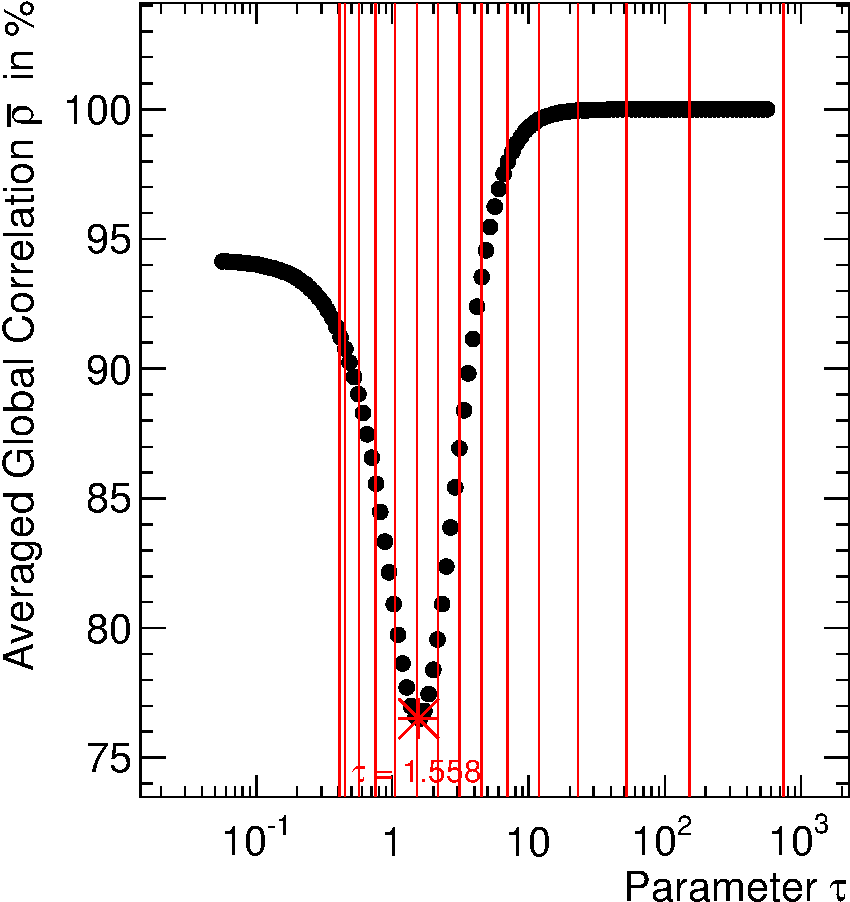
\includegraphics[width=5cm]{ExampleScan}
\par\end{centering}

\centering{}Example Plot for a $\tau$ scan using the averaged global
correlation $\rho$. The mimimum is clearly visible. The vertical
lines indicate the $\tau$ values corresponding to the possible choices
of the discrete $k$-parameter. 
\end{figure}

\par\end{center}


\lyxframeend{}


\lyxframeend{}\lyxframe{File Based Regularization}
\begin{itemize}
\item The results of the $\tau$ parameter scan are saved in a text file.

\begin{itemize}
\item The name of the text file is specified in parameter 'txtFile'.
\item The $\tau$ scan can be switched on by setting the third steering
option to 2.
\end{itemize}
\item For each distribution for which a $\tau$ scan is performed, a new
\textbf{line entry }will be appended to the file, containing:

\begin{itemize}
\item a \textbf{key} to identify the distribution.
\item the optimal regularization parameters.
\end{itemize}
\item Note: The file will never be overwritten!
\end{itemize}

\lyxframeend{}

 


\lyxframeend{}\lyxframe{File Based Regularization }
\begin{itemize}
\item Each line entry contains the following tokens (continued on next slide):

\begin{itemize}
\item \textbf{Key}: A string identifying the distribution under investigation.
The string is composed of the input parameters 'channel', 'particle',
'quantity' and (optionally) 'special' and has one of the two following
formats:

\begin{itemize}
\item <channel>\_<particle>\_<quantity>
\item <channel>\_<particle>\_<quantity>\_<special>
\end{itemize}
\item \textbf{Optimal $\boldsymbol{\tau}$ parameter}:\textbf{ }Optimal
$\tau$ parameter as determined from global correlation method.
\item \textbf{Closest lower $k$ parameter: }Highest of all k parameters,
which lead to softer regularization than the optimal $\tau$ parameter
as determined from global correlation method. 
\end{itemize}
\end{itemize}

\lyxframeend{}

 


\lyxframeend{}\lyxframe{File Based Regularization }
\begin{itemize}
\item Each line entry contains the following tokens (continuation from last
slide):

\begin{itemize}
\item \textbf{Closest higher $k$ parameter: }Lowest of all k parameters,
which lead to harder regularization than the optimal $\tau$ parameter
as determined from global correlation method.
\item \textbf{Optimal $k$ parameter: }Optimal k parameter as determined
from d-Value method.
\item \textbf{Optimal $k$ parameter: }Optimal k parameter as determined
from d-Value method.
\item \textbf{Number of Bins: }Number of generator level bins considered
in unfolding. This depends on the setting of steering options 10 and
11. 
\end{itemize}
\end{itemize}

\lyxframeend{}

 


\lyxframeend{}\lyxframe{File Based Regularization}
\begin{itemize}
\item A text file of the above format can be used as an input for file based
regularization.

\begin{itemize}
\item The name of the input text file is specified in parameter 'regParFile'
\item File based regularization is switched on by setting the first steering
option to 4.
\end{itemize}
\item For each distribution, the text file will be search for the \textbf{first
occurence of the corresponding key }and the regularization parameters
from the corresponding line entry will be parsed.
\item Note: Whether the optimal $\tau$ parameter from global correlation
method or the optimal k paramter from the d-Value method will be used,
depends on the setting of the first steering option.
\end{itemize}

\lyxframeend{}

 


\lyxframeend{}\lyxframe{Iterative Unfolding}
\begin{itemize}
\item TopSVDFunctions can be used iteratively. This refers to the following
procedure:

\begin{itemize}
\item Unfold the data with the nominal (unweighted) signal Monte Carlo.
\item Calculate generator level weights by comparing the unfolded data distribution
with the generated events.
\item Apply those generator level weights to the bins of the generator level
distribution and to the columns of the response matrix.
\item From the reweighted response matrix, calulate reconstruction level
weights. 
\item Apply those reconstruction level weights to the reconstructed distribution. 
\item Repeat these steps recursively, then perform final unfolding. 
\end{itemize}
\item Note: We do not reweight the data in any way! 
\item Iterative unfolding can be steered with steering option 15.
\end{itemize}

\lyxframeend{}

 


\lyxframeend{}\lyxframe{Latex Booklets with Control Plots}
\begin{itemize}
\item A zsh script \texttt{CP\_booklet/make\_CP\_booklet.sh }is provided
which

\begin{itemize}
\item groups \emph{same type} histograms together and
\item compiles and arranges them in a latex file.
\end{itemize}
\item Use this script, if 

\begin{itemize}
\item you unfold multiple distributions
\item and if you want to compare same type plots easily.
\end{itemize}
\item Check out the directory \texttt{CP\_booklet }which contains 

\begin{itemize}
\item the script \texttt{make\_CP\_booklet.sh,}
\item a README file,
\item A directory with sample steering files (ending: \texttt{.steer) and}
\item A directory with tex snippets used by the script.
\end{itemize}
\end{itemize}

\lyxframeend{}

 


\lyxframeend{}\lyxframe{Latex Booklets with Control Plots}
\begin{itemize}
\item Steering file syntax: For each booklet you want to create, you give
4 lines:

\begin{itemize}
\item The Extension of the EPS plots with which the filename ends. 

\begin{itemize}
\item Example: For plots with names like 'Unfolding\_<channel>\_<particle>\_<quantity>\_HAD\_InputDataGenRec.eps',
you should provide the 'InputDataGenRec'. Note, that his will also
be the name of the Tex/PDF file.
\end{itemize}
\item Whether this plot should be printed for the nominal sample or not
(\texttt{true} or \texttt{false}).
\item Whether this plot should be printed for the systematic samples or
not (\texttt{true} or \texttt{false}).
\item A descriptive title for the booklet in LateX Format 
\end{itemize}
\item The steering file is read successively, blank lines are ignored.
\end{itemize}

\lyxframeend{}

 


\lyxframeend{}\lyxframe{Latex Booklets with Control Plots}
\begin{itemize}
\item More steering options are hardcoded at the top of \texttt{make\_CP\_booklet.sh:}

\begin{itemize}
\item The output folder to use
\item the names of the systematics to loop over
\item the channels to loop over
\item the distributions to loop over (note, that this list is devided to
steer the distribution over two pages)
\item whether EPS should be converted to PDF (in case you want to use pdflatex)
\item whether the image files should be copied to a subdirectory of the
output folder
\item whether the tex files should be converted to PDF or not.
\end{itemize}
\end{itemize}

\lyxframeend{}

 


\lyxframeend{}\lyxframe{Latex Booklets with Control Plots}
\begin{itemize}
\item Example steering:


\texttt{InputResponseMatrix }


\texttt{true }


\texttt{false }


\texttt{Probability Matrix \$\textbackslash{}mathrm\{\textbackslash{}boldsymbol\{M\}\}\$}

\item This creates a latex booklet ``InputResponseMatrix.tex'' with all
nominal response matrices, but no systematics reponse matrices.
\end{itemize}

\lyxframeend{}
\end{document}
